\chapter{INTERFACE DEVELOPED FOR THE BLENDER GAME ENGIME}\label{chap5}

% introduction

% video game history
Video games have been around since the 1950s\cite{historyVideoGames}. They became available on the marketplace by the 1970s, at which time they were very popular. Currently, games are ubiquitous, played by people of all ages, and a wide range of electronic devices. Current video games run on specialized consoles, portable consoles, desktop and mobile computers, even phones. It is hardly possible to go through the day without being in contact, directly or indirectly with some kind of video game.

% our aim
Our aim is to develop tools that would help to create \textit{educational} games. Educational games are played for enjoyment, but also for their ability to teach something to the player. 

% layout of the chapter
This chapter starts with a brief discussion of \textit{Blender}, followed by a description of its \textit{Game Engine}. We then cover the standalone Boids particle system of Blender, and finally, we describe the flocking modifier that has been integrated into the Blender Game Engine. 


% blender background info
\section{Blender}\label{blenderSec}
\textit{Blender}\cite{blenderWeb} is a free modeling/simulation software, available since 1993. Originally meant for the creation of 2D and 3D content, it has been significantly extend to handle modeling, texturing, animation, particle simulation, rendering, game creation, and more. 

When searching for the right software to use, the following features were considered important: inclusion of a game engine, extendability, open source, cross-platform, has a physics engine, and has a very large support based. Blender satisfied all the above criteria. The Blender release used in this thesis was 2.57.

% game engine
\section{Game Engines}

% what is a game engine?
A game engine is a software or part of a software that simulates virtual reality\cite{bookGameKit2}. Modern game engines provide real-time interaction with a make-believe world, including controlling objects, letting them interact with the environment, and with the player. 

Game engines have several tasks:
\begin{enumerate}
\item{render the 3D world and the objects in it}
\item{re-render the scenes when something in the world changes}
\item{make decisions during gameplay using a logic engine}
\item{simulate the physics of the game world i.e. gravity}
\item{handle collision detection and reaction to collisions}
\end{enumerate}

Game engines try to simulate the scenes as quickly as possible, so the game has a smooth fluency. Game engines are much more complicated than this, these are just a few of the most important jobs that characterize them.

% blender game engine
The Blender Game Engine is a very powerful tool, allowing the creation of simple games without  the need for explicit programming. With its GUI one can create simple games using a graphical logical editor, which has a click and drag interface, shown in Figure~\ref{logic}. Each object in the scene has logical components associated to it. 

\begin{figure}[htbp]
\begin{center}$
\begin{array}{c}
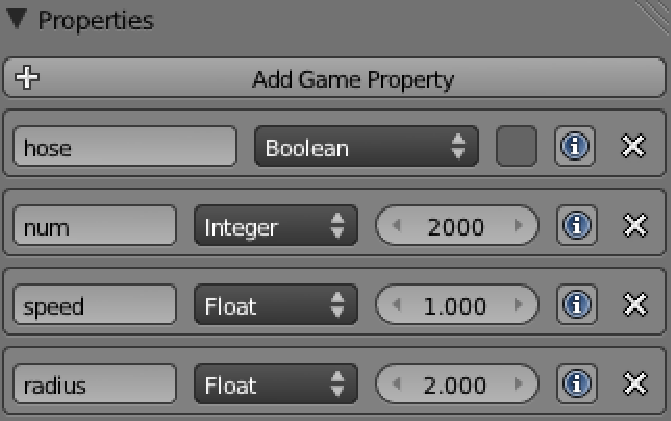
\includegraphics[scale=0.5]{figures/logic_properties.pdf} \\
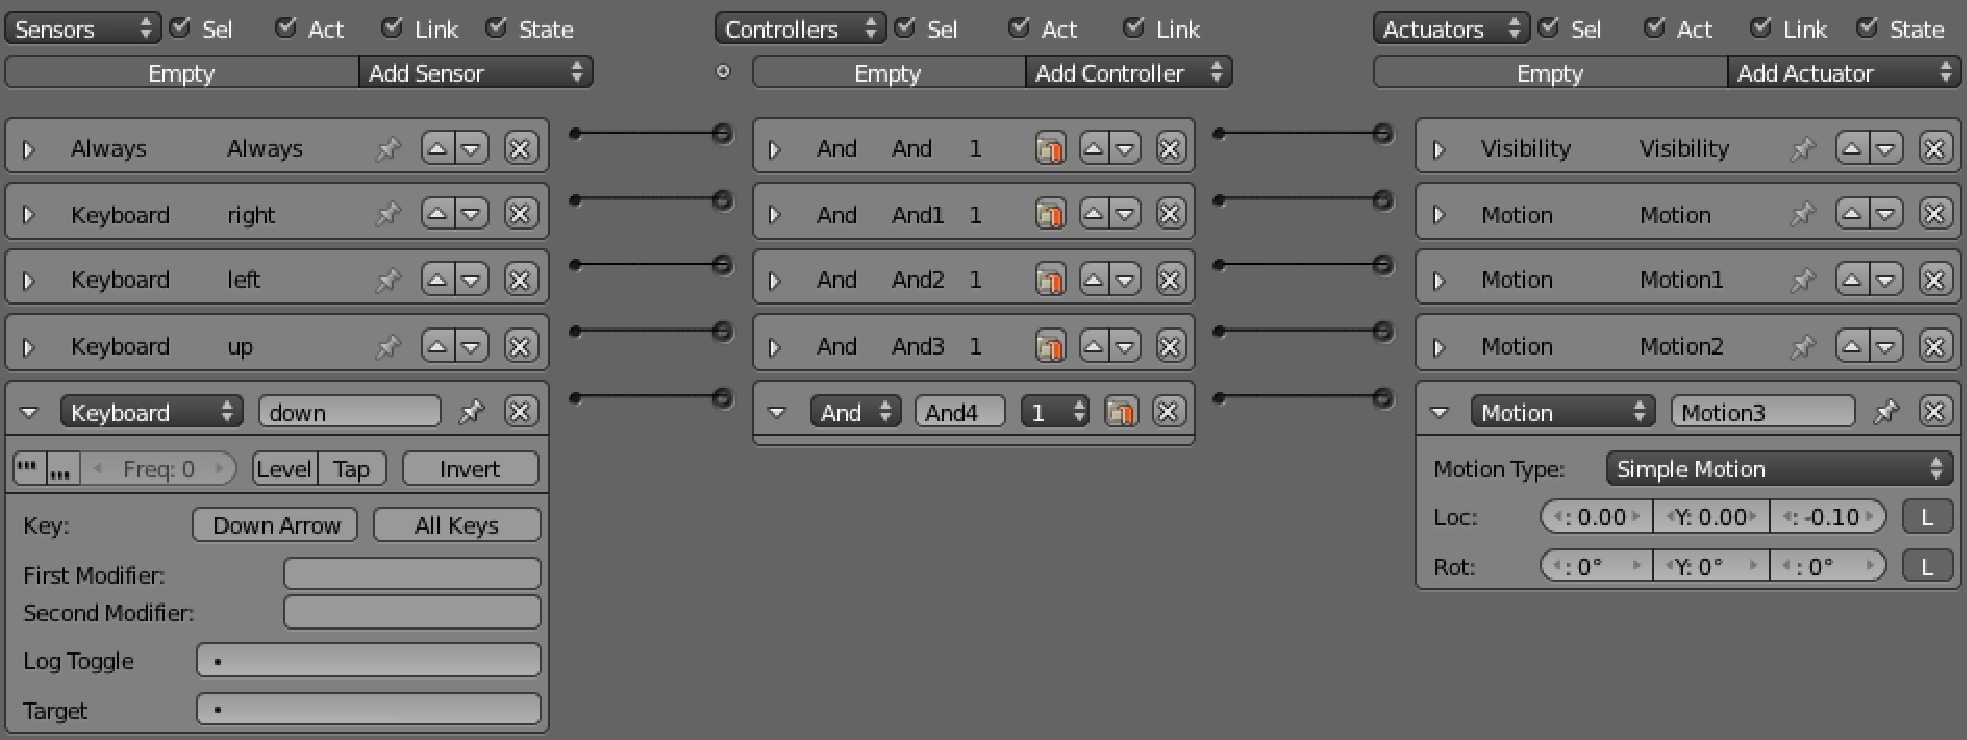
\includegraphics[scale=0.45]{figures/logic_bricks.pdf}
\end{array}$
\end{center}
\caption{The Blender Game Engine Logic Editor interface: consists of Properties and Logic Bricks}
\label{logic}
\end{figure}

The logic editor interface consists of two parts: \textit{Properties} and \textit{Logic Bricks}. Properties are used to provide objects with additional specific actions. These properties can be accessed by name either through the logic editor or through python programming. In the second part, the logic bricks are divided into \textit{sensors}, \textit{controllers}, and \textit{actuators}. Each class of bricks has different subtypes to chose from.

Sensors are used to detect the input from the user, e.g. keyboard, mouse, joysticks, etc. Controllers link the Sensors to the Actuators. Controllers provide the logic that determines action taken by the actuators. For example, the object might move, rotate, create, destroy, change 
shape, etc.

Object logic is formed from as many logic bricks as necessary. The bricks are interconnected: sensors to controllers and controllers to actuators. The properties in Figure~\ref{logic} shows a setup of a hose emitter, the logic bricks show the configuration that leads to the movement of a cube using the arrows.

The logic editor is the simplest approach creating objects that interact in the gameworld. More Complex behavior is possible through the Python scripting interface.

% particle system outside the blender game engine
\section{Boids Particle System outside the Blender Game Engine}
Although Blender has extensive particle-based tools, including hair styling, these are absent from the Game Engine. A submodule of the particle system is a rather sophisticated Boids system. This Section presents a demonstration to illustrate the functionality of the built-in Boids system. 

One initially creates a particle emitter, such as a cube, a plane, or other object. Then, make that object into a particle system. Figure~\ref{boidsCreatePS} shows the panel used to add the particle system. The number of particles is initially set to 50. The lifetime of the boids is set to a large number.

% figure: create PS
\begin{figure}[htbp]
\begin{center}
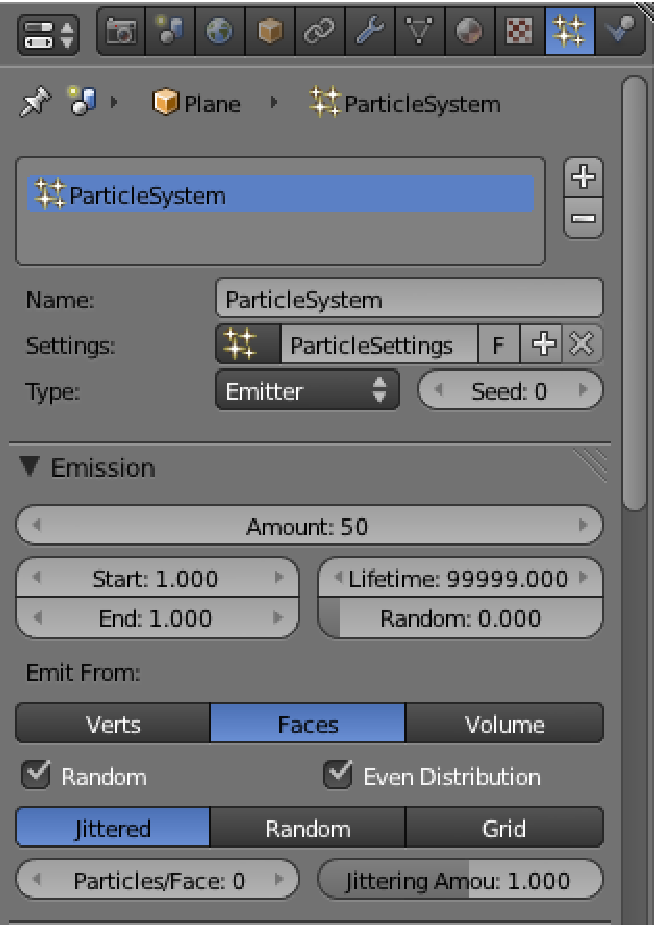
\includegraphics[scale= 0.65]{figures/boidsCreatePS.pdf} 
\caption{Blender Particle Systems Add and Emission panels: add a particle system and set the number of particles in that particle system}
\label{boidsCreatePS}
\end{center}
\end{figure}

After the system is created, the physics of the system can be edited, see Figure~\ref{boidsPhysics}. The \textit{Boids} button takes the user to a panel with all the settings of the Boid system.  Note that the settings can be changed dynamically during the animation. 

% figure: boids physics
\begin{figure}[htbp]
\begin{center}
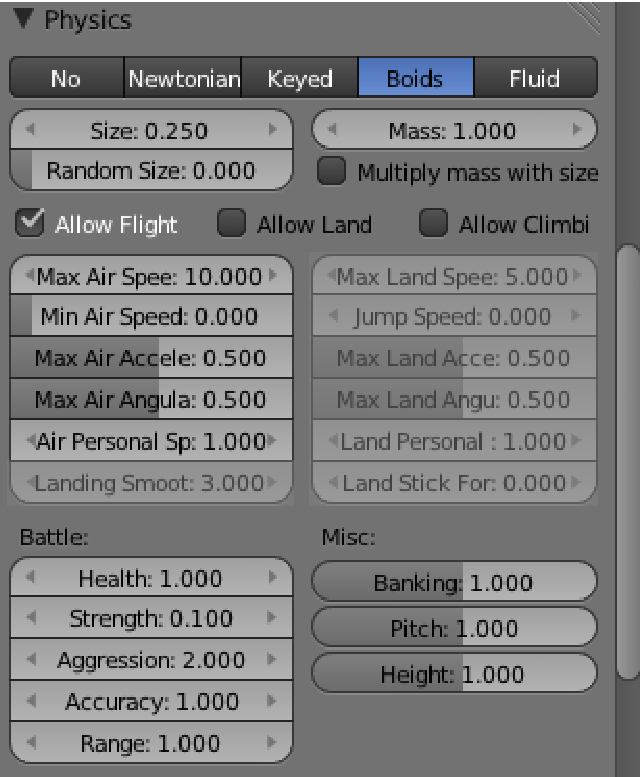
\includegraphics[scale = 0.65]{figures/boidsPhysics.pdf} 
\caption{Blender Particle Systems Physics panel for Boids: set the physical properties of the Boids particle system}
\label{boidsPhysics}
\end{center}
\end{figure}

In the Blender Boids system, the boids have their own brain; therefore more specific settings can be assigned depending on the application. Figure~\ref{boidsBrain} shows the panel for the Boids Brain (a Blender label). In this panel, one finds the rules available to the boids\footnote{Description of rules is listed as it is in the Blender source code.}.

%Blender boid's rules
\begin{enumerate}
\item{\textit{Goal}: go to the goal assigned object or loudest assigned signal source}
\item{\textit{Avoid}: get away from assigned object or loudest assigned signal source}
\item{\textit{Avoid Collision}: maneuver to avoid collisions with other boids and deflector object in near future}
\item{\textit{Separate}: keep from going through other boids}
\item{\textit{Flock}: move to center of neighbors and match their velocity}
\item{\textit{Follow Leader}: follow a boid or assigned object}
\item{\textit{Average Speed}: maintain speed, flight level or wander}
\item{\textit{Fight}: go to closest enemy and attack when in range}
\end{enumerate}

When clicking in a rule, parameter panels appear if needed. As seen in Figure~\ref{boidsBrain}, clicking the rule \textit{Goal} leads to an the option to set the object which is the boid target. The figure shows an empty object we created. 

There are three methods available in Blender to evaluate the rules: 1) fuzzy logic with a fuzziness level, 2) averaging all the rules, and 3) weighting the rules randomly. Each of these evaluation methods leads to completely different results. The default method of rules evaluation is Fuzzy.

The render panel, also seen in Figure~\ref{boidsBrain} shows the options for rendering the flock. We changed the rendering type to object and specified that each boid be rendered as a monkey object.

% figure: boid brain
\begin{figure}[htbp]
\begin{center}
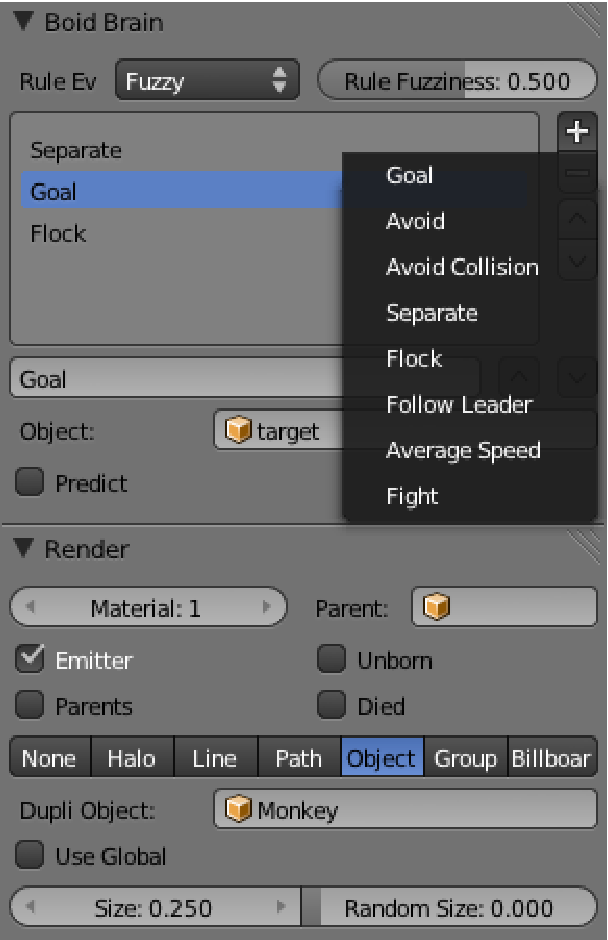
\includegraphics[scale = 0.65]{figures/boidsBrain.pdf}
\caption{Blender Particle Systems Boid Brain and Render panels: set the rules that boids are going to follow, and set the render type}
\label{boidsBrain}
\end{center}
\end{figure}

Figure~\ref{boidsAction} shows two screenshots of an animation in which the boids are approaching an empty object as the target. This animation was run using the settings presented in the previous Figures.

% figure: boids in action
\begin{figure}[htbp]
\begin{center}$
\begin{array}{cc}
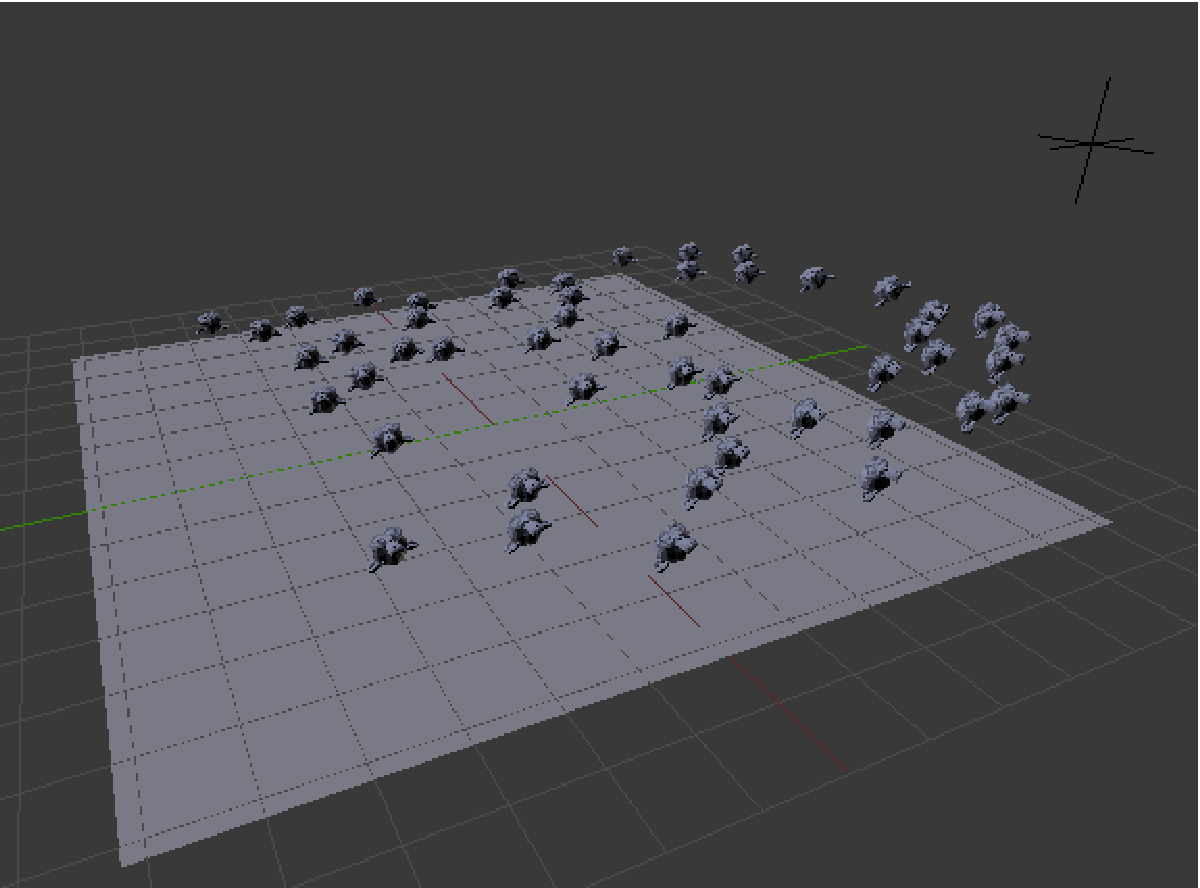
\includegraphics[scale= 0.35]{figures/boids1.pdf} &
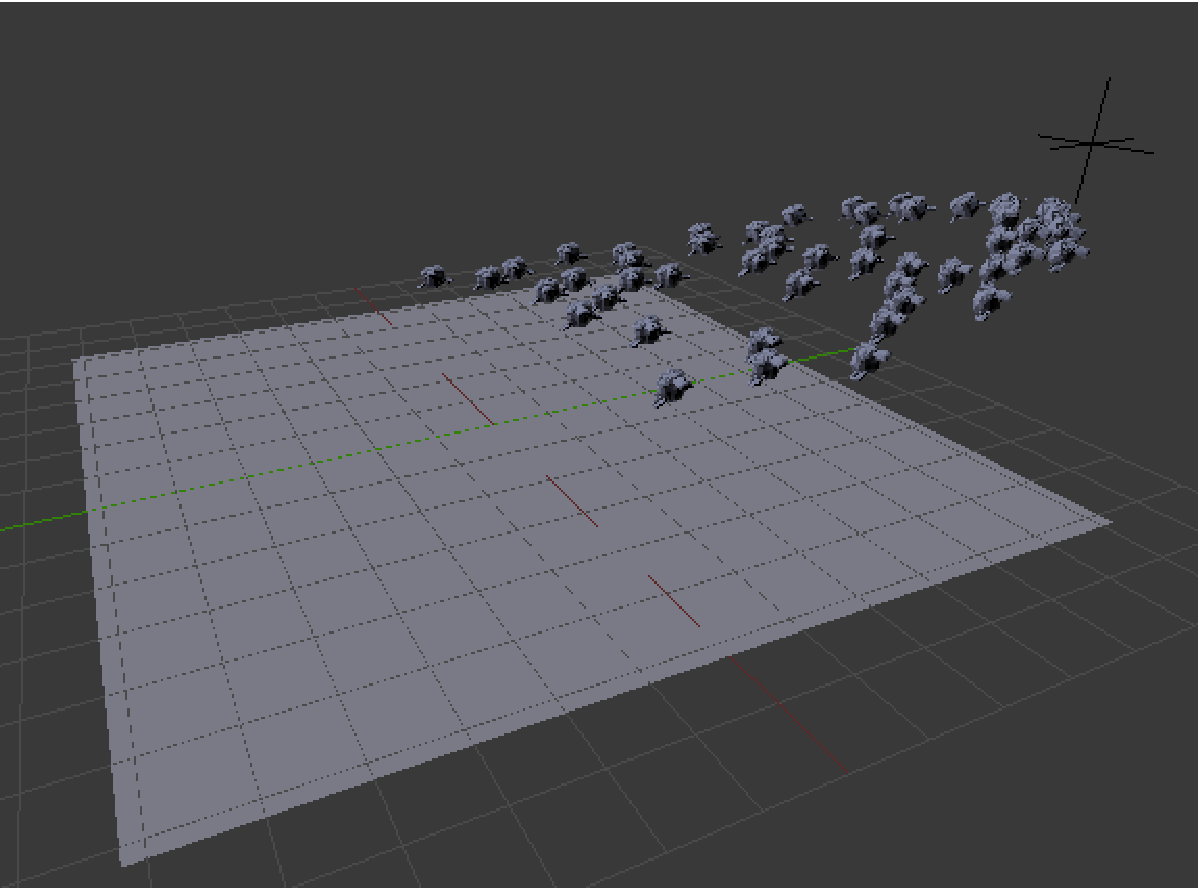
\includegraphics[scale= 0.35]{figures/boids2.pdf}
\end{array}$
\end{center}
\caption{Screenshots of the boids approaching the target i.e. an empty object. }
\label{boidsAction}
\end{figure}

% RTPS modifier
\section{RTPS Modifier}\label{modifiersection}
We now present the interface developed to link the Blender Game Engine with our FLOCK system defined in the RTPS library. Blender modifiers are ideally suited to this task. They are used to edit the object through the assignment of properties. For example in our case, first we create the domain using a Blender cube and then assign the RTPS modifier to it. 

For a step by step description on how this modifier was created, see Ian Johnson post at \url{http://enja.org/2010/05/24/blender-creating-a-custom-modifier/}.  The functionality of the Boids system was added to the original RTPS modifier which was created to support only SPH systems. 

% code modifications
\subsection{Game Engine Source Code Modifications}
The creation of the custom modifier involved modifying a few files. These modifications fell into three categories: Functionality of the Game Engine, Functionality of the UI Modifier, and  Creation of the UI Modifier.

The main changes made to the Blender source code are summarized in Tables~\ref{geTable},~\ref{funcTable},~\ref{uiTable}.

% tables summarizing the changes made to the source code

% GE table
\begin{table}[htdp]
\caption{Modifications made for the functionality of the Game Engine}
\begin{center}
\begin{tabular}{|p{6cm}|p{6cm}|}
\hline 
\textbf{File} & \textbf{Summary of the Modifications} \\\hline 
BL\_BlenderDataConversion.cpp & Checks if the RTPS modifier is in use. \\\hline 
BL\_ModifierDeformer.cpp & Implementation of the RTPS functionality inside Blender. The RTPS object is created and updated. \\\hline 
RAS\_ListRasterizer.cpp & Calls the \texttt{render()} method. \\
\hline 
\end{tabular} 
\end{center}
\label{geTable}
\end{table}

% Functionality table
\begin{table}[htdp]
\caption{Modifications made to the functionality of the UI modifier}
\begin{center}
\begin{tabular}{|p{6cm}|p{6cm}|}
\hline 
\textbf{File} & \textbf{Summary of the Modifications} \\\hline 
DNA\_modifier\_types.h & Defines the \texttt{struct} of the RTPS modifier. \\\hline 
rna\_modifer.c & Defines the properties of the items in the UI. \\\hline 
MOD\_rtps.c & This file was created and defines the default values of the parameters in the UI. \\
\hline 
\end{tabular}
\end{center}
\label{funcTable}
\end{table}

% UI table
\begin{table}[htdp]
\caption{Modifications made for the creation of the UI modifier}
\begin{center}
\begin{tabular}{|p{6cm}|p{6cm}|}
\hline 
\textbf{File} & \textbf{Summary of the Modifications} \\\hline 
properties\_data\_modifier.py & Creates the UI modifier using the properties defined in \texttt{rna\_modifier.c}. \\
\hline 
\end{tabular}
\end{center}
\label{uiTable}
\end{table}

% UI description
\subsection{Development of the UI}
Our RTPS modifier as the Blender interface is implemented using \textit{Python}. As described in table~\ref{uiTable} the only file modified for the development of the UI was \texttt{properties\_data\_modifier.py}. The RTPS modifier is shown in Figure~\ref{ui}.

% figure: RTPS modifier
\begin{figure}[htbp]
\begin{center}
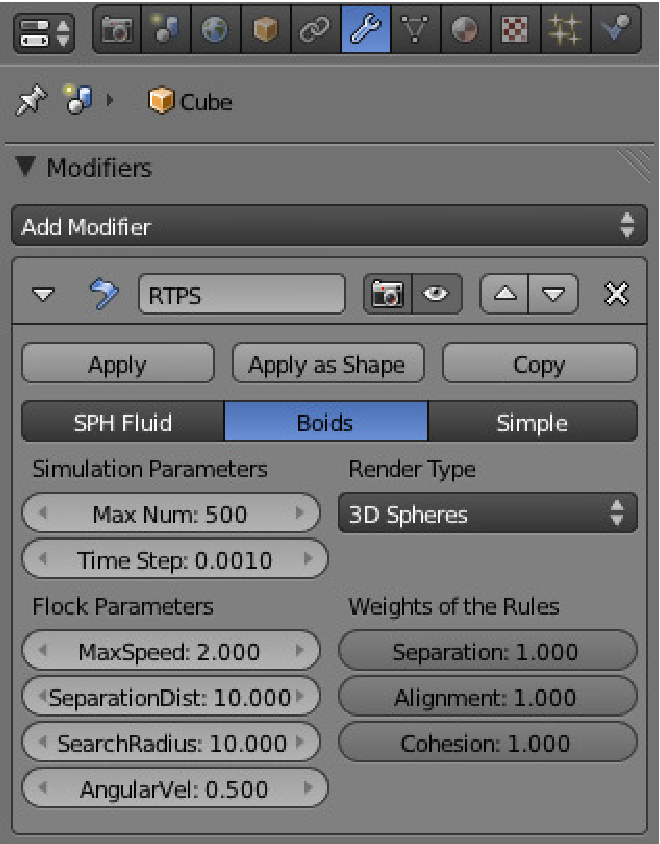
\includegraphics[scale=0.8]{figures/modifier.pdf}
\caption{Boids system of the RTPS modifier: it includes the simulation parameters, the render types, the flock specific parameters, and the scalar weights for each of the rules; here showing the default values}
\label{ui}
\end{center}
\end{figure}

The RTPS modifier is used to initialize the particle systems available in the RTPS library by assigning certain properties to the Blender object. The Boids system in the RTPS modifier includes several simuliation parameters (the maximum number of particles, the time step used for integration, and the option for 2D flocking), Render types (render the boids as Points, Sprites, Screen Space, and 3D Spheres). The color used to render the particles is computed  from the Blender's materials.

The Flock Parameters area presents the user with control over the maximum speed of the boids, the minimum separation distance between boids and the searching radius for the neighbor search. One can specify the various scalar weights of Equation~\ref{combine}, in the Weights of the Rules area.

\textit{How does the RTPS modifier works internally?} The modifier is applied to the object when the game engine starts. When the RTPS modifier is applied the RTPS object is created and initialized the RTPS object using the current parameters in the modifier interface. Once created, the RTPS object is updated, once per frame. 
%The object is updated at every frame.    

\textit{How to emit particles into the system?} There are two emitters available in the RTPS modifier: \textit{Blob} and \textit{Hose}. One uses these emitters by setting their respective properties (see Table~\ref{properties}). \textit{Blob} has the single associated property \texttt{num}, while the \textit{Hose} emitter is controlled via the three properties \texttt{num}, \texttt{speed}, and \texttt{radius}. The direction in which the particles are emitted when using the \textit{Hose} is determined by the \textit{y-axis} of the emitter object. 

% properties table
\begin{table}[htdp]
\caption{Properties available in the RTPS modifer}
\begin{center}
\begin{tabular}{|p{3cm}|p{9cm}|}
\hline 
\textbf{Property} & \textbf{Type and Description} \\\hline 
\texttt{num} 	& \texttt{integer}: if num $>$ 0, num particles are emitted every frame and num is reset to 0	\\\hline 
\texttt{hose}	& \texttt{boolean}: used to active the hose	\\\hline
\texttt{speed}	& \texttt{float}: initial velocity of the particles emitted from the hose	\\\hline
\texttt{radius}	& \texttt{float}: width of the hose	\\ %\hline
%\texttt{index}	& \texttt{integer}: used when more than hose is been used in the game	\\\hline
%\texttt{refill}	& \texttt{integer}: 	refill the hose \\\hline
%\texttt{collider}	& \texttt{boolean}: used to active collisions detections in the SPH system	\\
\hline 
\end{tabular}
\end{center}
\label{properties}
\end{table}

